\section{Discusión}

Una vez que se han conseguido los resultados correspondientes, se procede a discutir los diferentes problemas y hallazgos en esta sección

\subsection{Análisis inicial de genes y proteínas}

\subsubsection{Red PPI SARS-Cov2}

La red de interacción entre proteínas del SARS-Cov2 se compone de un total de \emph{332 proteínas cebo del virus que interactúan con el organismo humano}. Una proteína cebo es aquella que se usa para identificar las interacciones de las otras proteínas que nos interesa analizar (conocidas como \textit{proteínas cebo}). Suelen ser elegidas aquellas de las que se dispone información 

\newline

La red mostrada a continuación muestra un esquema de colores que identifican aquellas proteínas que participan en una misma interacción viral. En la figura se muestran las 10 proteínas con mayor interacción entre ellas así como otras 15 adicionales que, según Uniprot, son relevantes para la enfermedad. Tenemos un total de \emph{25 proteínas} que forman un total de \emph{61 interacciones} a nivel global de red con una media aproximada de \emph{grado de 4.88}.El \textit{p} valor es prácticamente nulo \textit{(0.000173}:

	\begin{figure}[h!]
		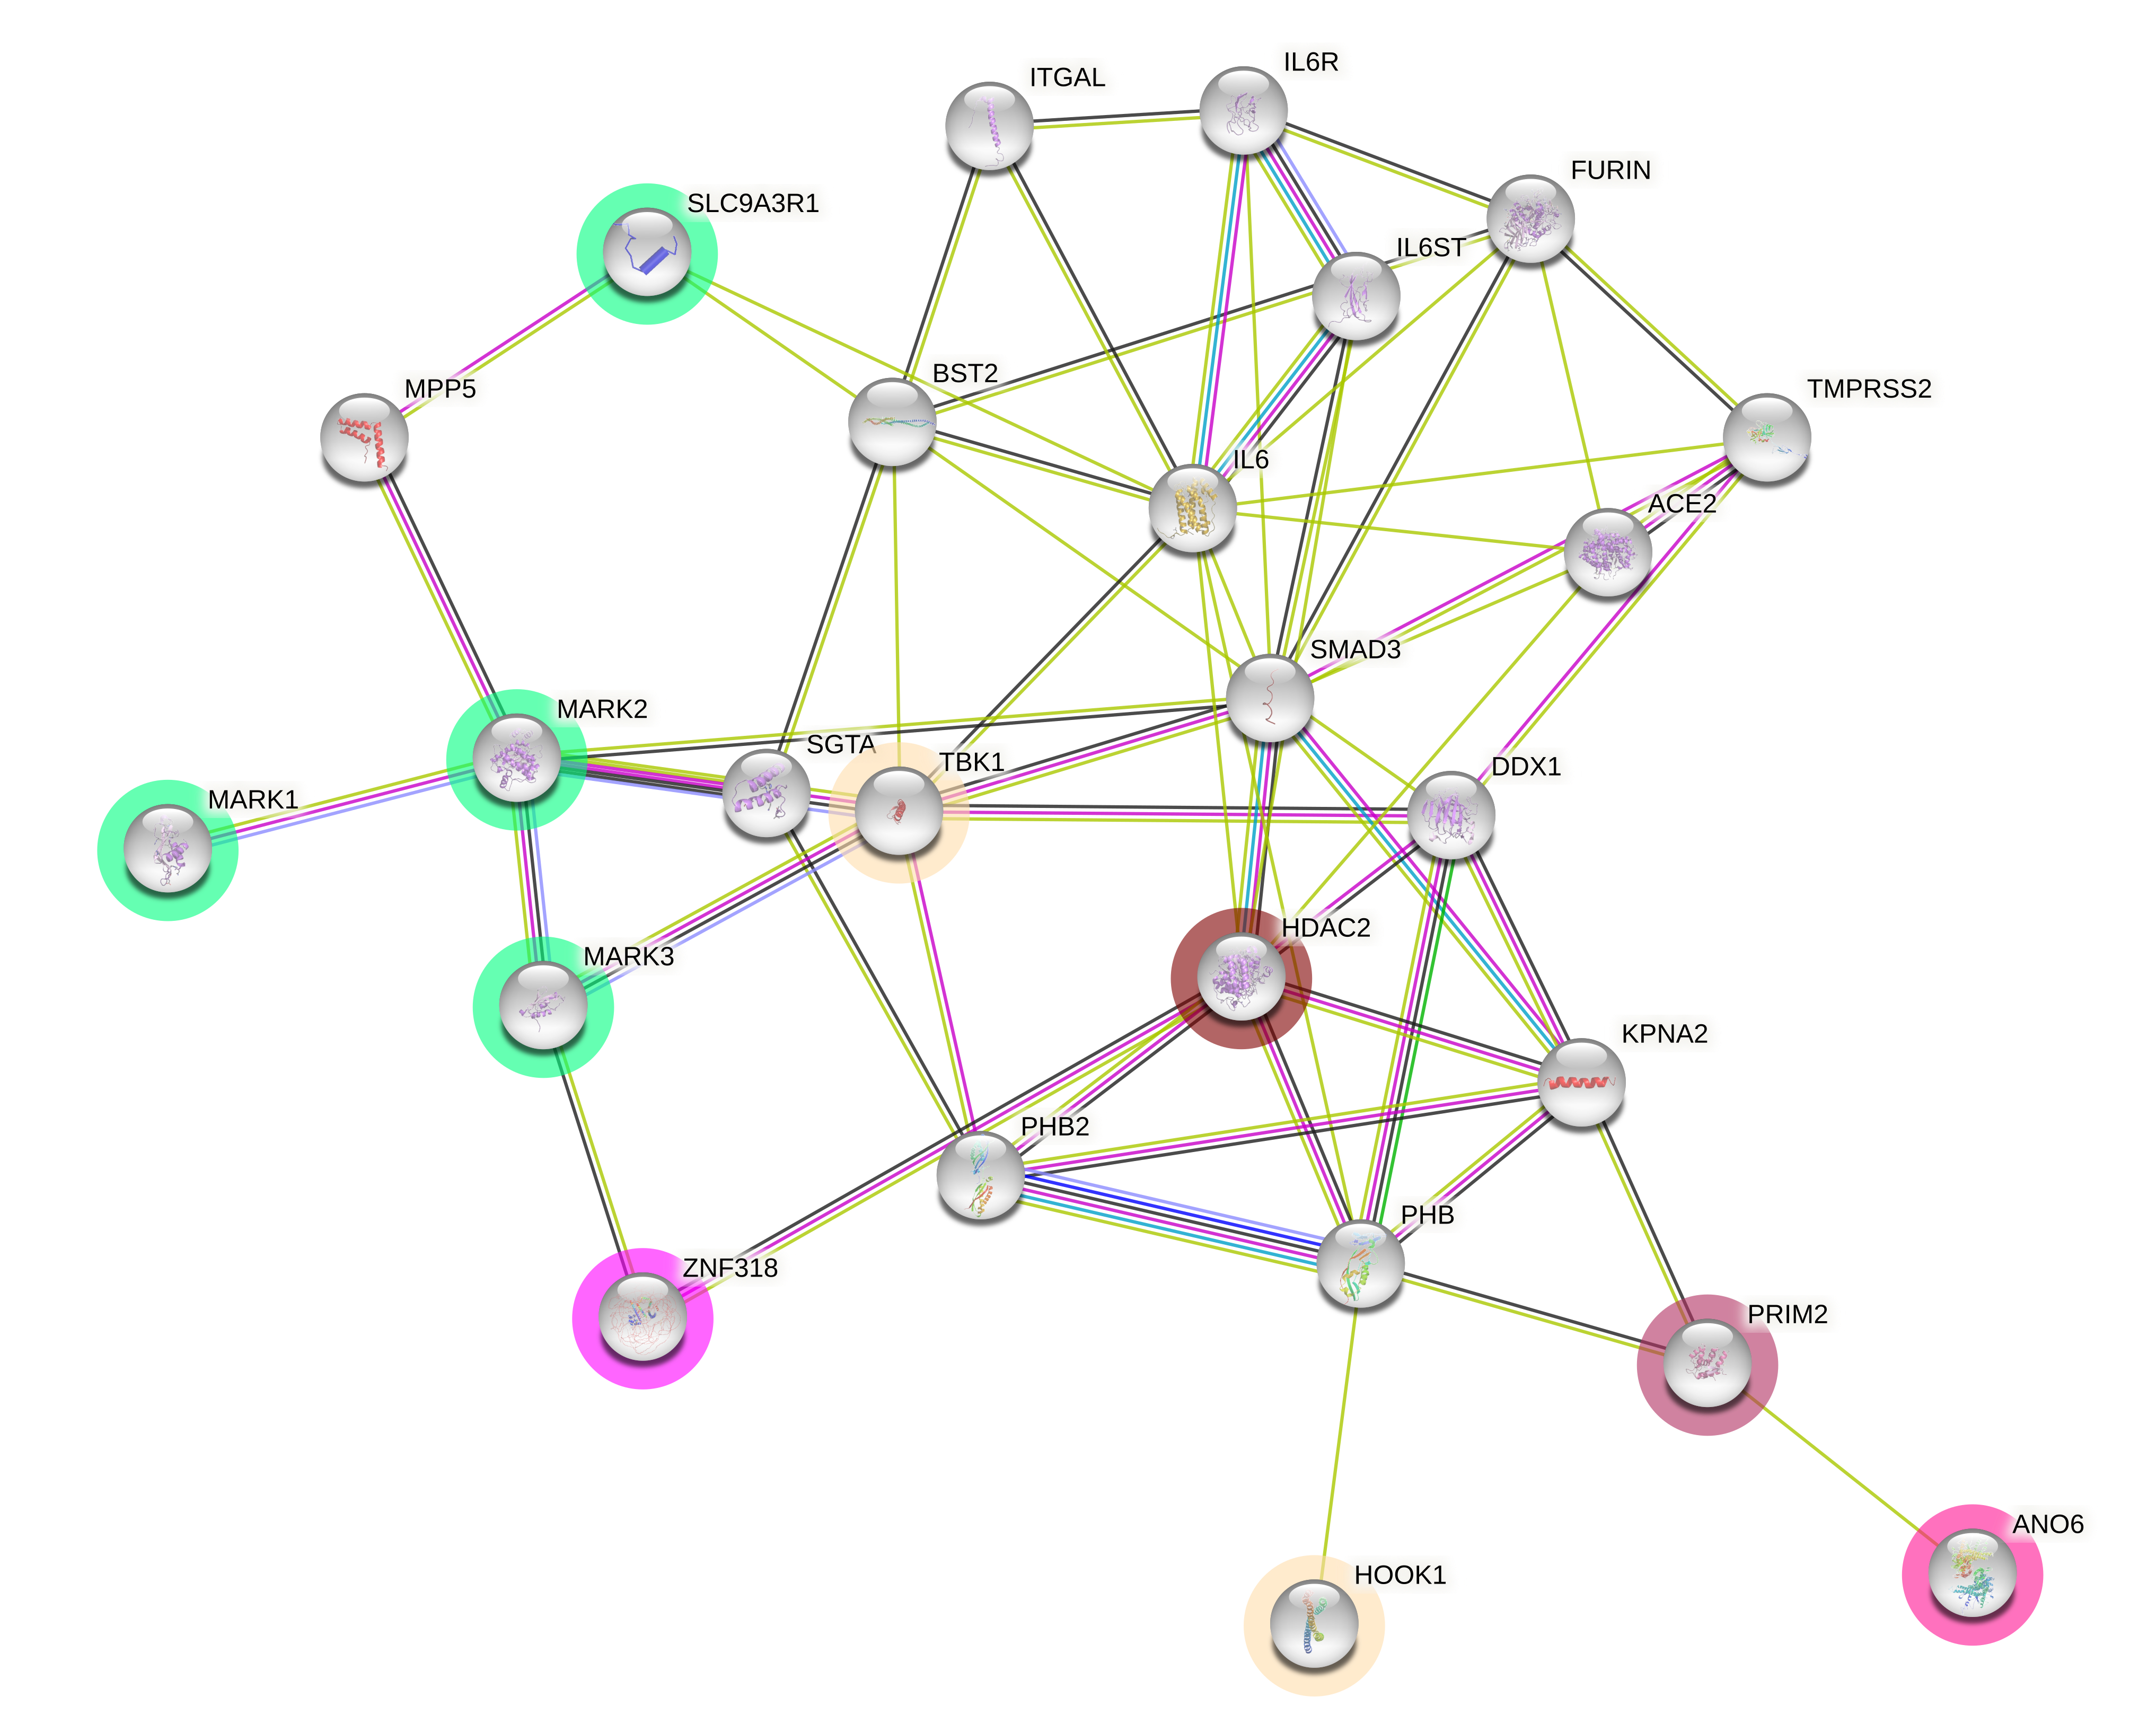
\includegraphics[width=0.9\textwidth]{figures/PPInetSARSCov2BaitProt.png}
		\caption{SARS-CoV-2 protein interaction map}
		\label{fig:ppi_net}
	\end{figure}
	
	\begin{figure}[h!]
		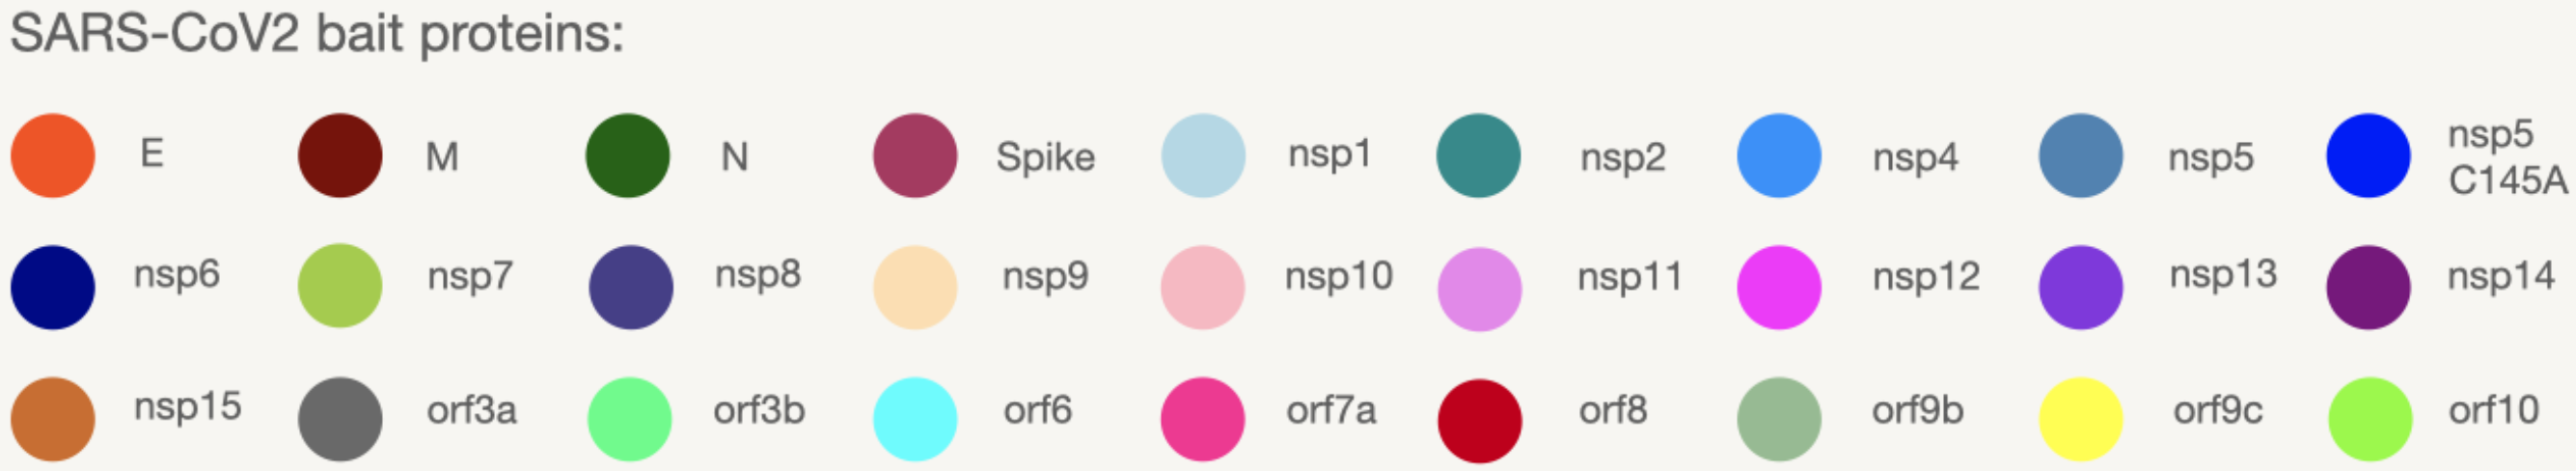
\includegraphics[width=0.9\textwidth]{figures/PPIColourLegend.png}
		\caption{Colour Legend}
		\label{fig:ppi_legend}
	\end{figure}

Se procede a descargar la información casi completa de toda la red (246 de las 332 proteínas) en forma de archivos \textit{tsv} para su posterior lectura y graficación usando código en \textit{R}. Se observa que, del total, tan sólo \emph{existen interacciones significativas entre 67 proteínas cuando originalmente se esperaban 4 interacciones} a nivel global de la red. El elevado número de interacciones nos indica que esta red no es fruto del azar(como prueba el \textit{p} valor de 0), si no que se trata de un red real e indicativo de que las proteínas probablemente están asociadas a funciones biológicas.

	\begin{figure}[h!]
		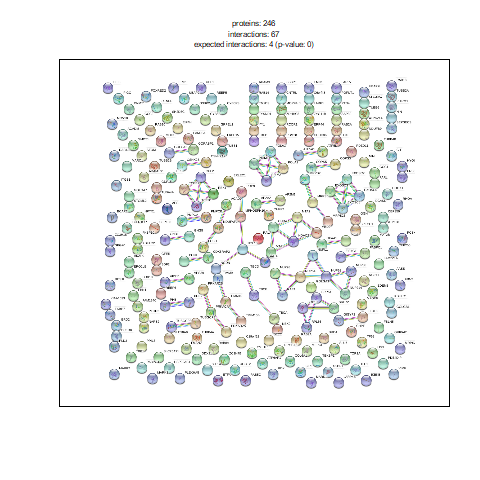
\includegraphics[width=0.9\textwidth]{../results/figuraSTRINGdb.png}
		\caption{Full protein interaction map}
		\label{fig:ppi_stringdb}
	\end{figure}

Ahora se tiene la absoluta certeza de que estas proteínas pueden estar asociadas entre sí y, por lo tanto, posiblemente puedan estar relacionadas con otras patologías a través de sus fenotipos.
	
\subsection{Análisis de comorbilidades}

Usando los datos recopilados en el archivo \textit{nodes&diseases.tsv} en el que se encuentran asociadas las proteínas y sus posibles enfermedades derivadas, se puede visualizar el subconjunto de aquellas que filas que contenga una proteína y su enfermedad (se desechan aquellas con las que no se tenga información de su patología correspondiente). La red resultante de \textit{iGraph} de 75 nodos queda de la siguiente forma:

	\begin{figure}[h!]
		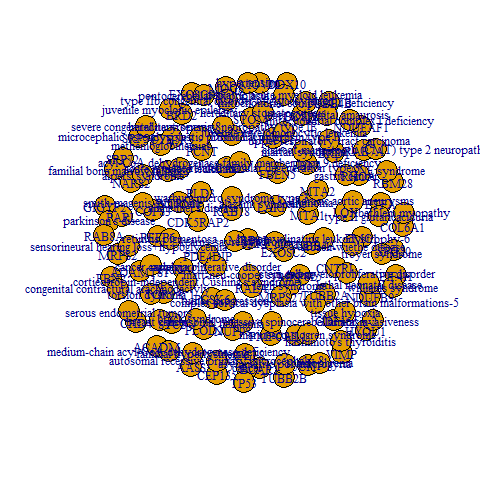
\includegraphics[width=0.9\textwidth]{../results/figuraiGraph.png}
		\caption{Partial protein-disease network (iGraph)}
		\label{fig:ppi_sigraph}
	\end{figure}
	
Aunque algo desordenada, se puede apreciar que hay enfermedades que hay nodos de tipo \textit{proteína} y nodos del tipo \textit{enfermedad} (sin diferencias visuales aparentes). Aquellos nodos que se encuentren más cercanos entre sí guardan una relación y viceversa. Se decide probar una nueva y mejor representación usando el paquete \texit{R} de \texit{linkcomm}. Se encuentran nodos más grandes que otros, indicativo de un grado superior y su mayor nivel de conectividad. Estos nodos coinciden con proteínas, con lo que se deduce que \emph{una importante minoría de proteínas están relacionadas con más de una patología} u otra proteína con su patología correspondiente. Podemos destacar \texit{COL6A1,  ACLADM y la PMCA }, aunque también se ve una enfermedad que está asociada a varias proteínas.

	\begin{figure}[h!]
		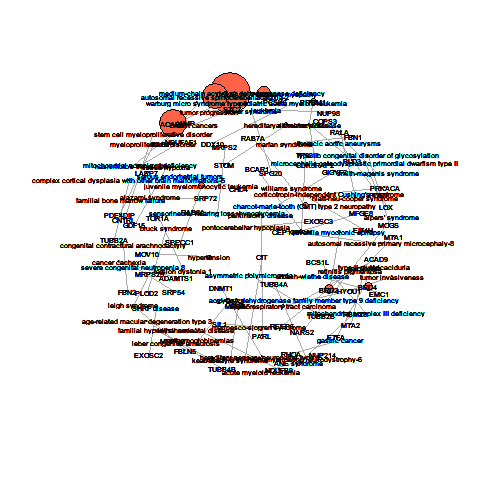
\includegraphics[width=0.9\textwidth]{../results/figuraLinkcomm.png}
		\caption{Partial protein-disease network (linkcomm)}
		\label{fig:ppi_linkcomm}
	\end{figure}
	
Tal como se puede ver, \emph{se ha logrado un mapa con cierto nivel de detalle sobre las diferentes comorbilidades del SARS-Cov2} usando diferentes paquetes de modelado de redes con \textit{R (stringdb, iGraph, linkcomm}. Se han podido analizar las redes, confirmando las interacciones entre proteínas así como las relaciones que existen con diferentes patologías.